\section*{Exercice 158 -- SED}
(Pôle Chateaubriand Joliot Curie)

\setcounter{exo}{0}


Dans l’objectif d’optimiser le fonctionnement d’un hydro-planeur il faut tenir compte de toutes les procédures de fonctionnement prévues, comme celle d’alerte en cas de panne de la transmission des données, qui impose d’émettre un signal de détresse permettant de venir repêcher l’hydro-planeur.
À chaque remontée en surface, l’hydro-planeur se connecte à un réseau sans fil (IRIDIUM) afin de transmettre les données enregistrées. L'hydro-planeur dispose de trois antennes logées dans la dérive et dans chaque aileron stabilisateur. Cette solution implique que, pour émettre en surface, l’engin pivote sur lui-même d’un quart de tour pour faire émerger une des deux antennes dédiées au réseau IRIDIUM. Pendant cette phase, le dispositif de basculement, qui permet de contrôler le tangage de l’hydro-planeur, n’est pas actif.
En fin de charge des batteries ou en cas de souci technique, l’hydro-planeur dispose d’une balise ARGOS (dont l'antenne est dans la dérive verticale) qui permet de le localiser et d’envoyer un navire pour le récupérer.

\begin{center}
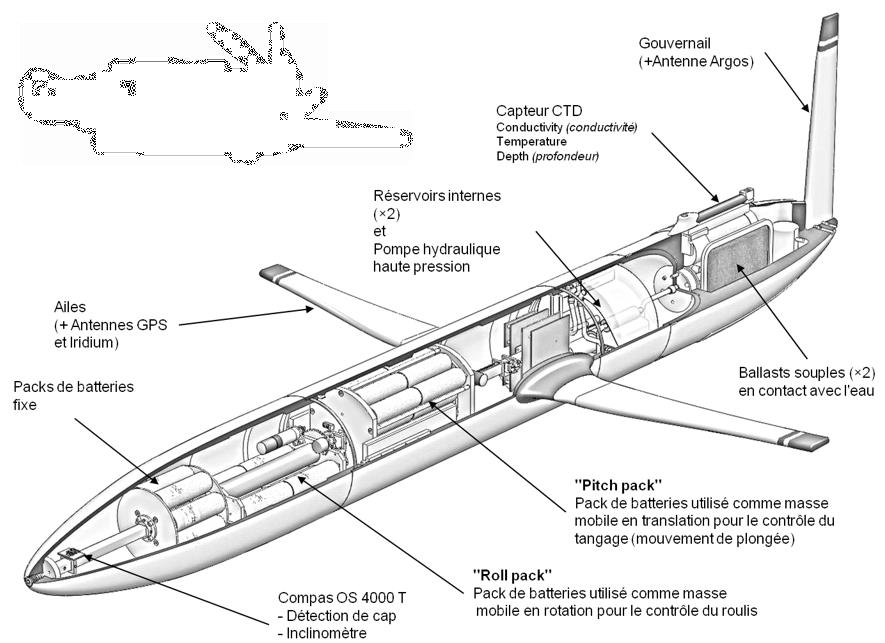
\includegraphics[width=\linewidth]{059_01}
\end{center}


\begin{center}
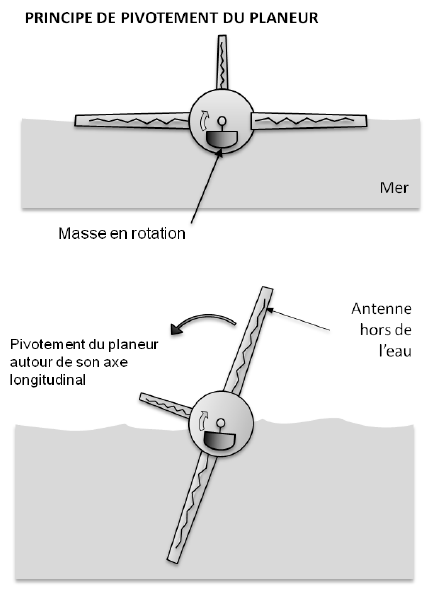
\includegraphics[width=\linewidth]{059_02}
\end{center}

Dans ce cas de dysfonctionnement, l’hydro-planeur adopte le comportement décrit par le diagramme d’état ci-dessous :


\begin{center}
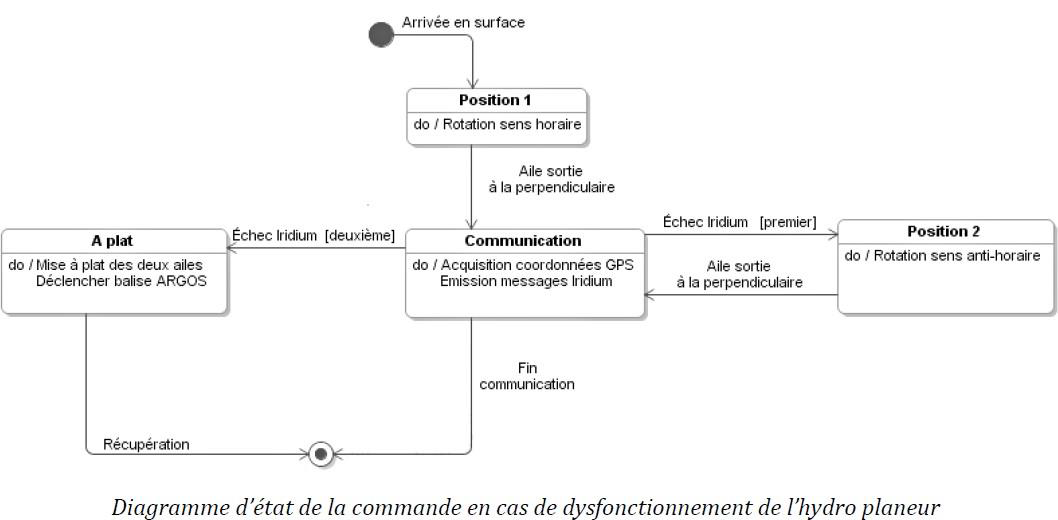
\includegraphics[width=\linewidth]{059_03}
\end{center}

\subparagraph{}
\textit{Compléter les chronogrammes qui correspondent à la séquence des signaux de commande fournis par l’unité de traitement pour obtenir le fonctionnement souhaité dans le cas où la première et la deuxième transmission IRIDIUM échouent (lorsqu’un élément doit être activé, il sera représenté par un niveau haut).}

\begin{center}
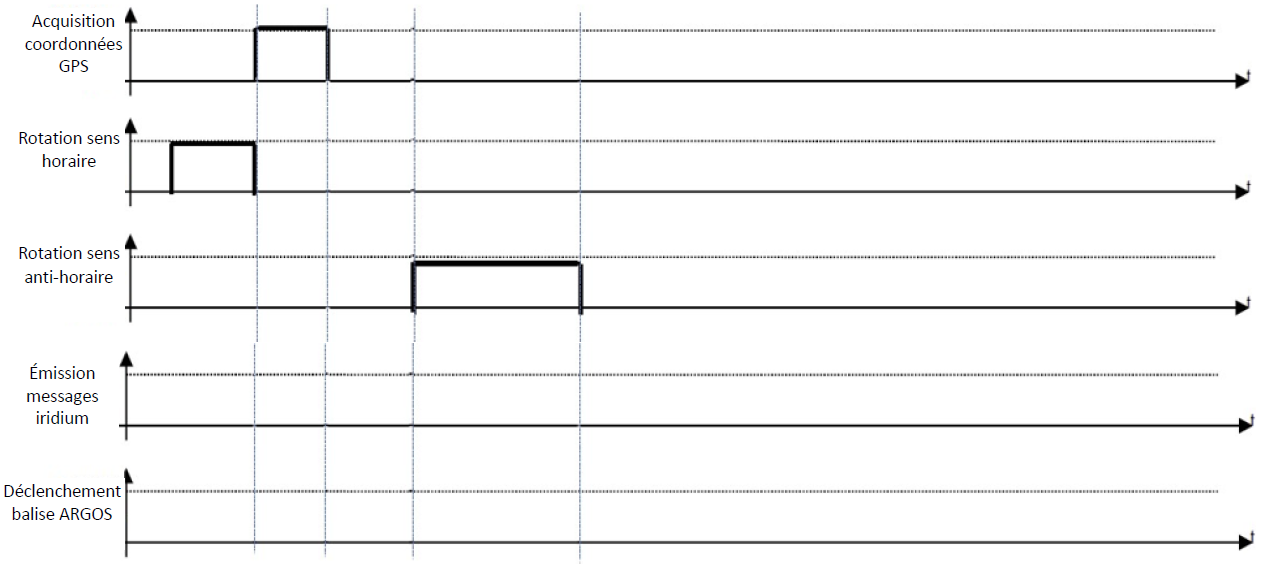
\includegraphics[width=\linewidth]{059_04}
\end{center}